% ============================================================
% 分片：s02h  对应原文 PDF 第 29--32 页（并含第 33 页页首的那个跨页句）
% 负责章节：2.4.3 $A$-branes and the Fukaya category（至 §3 之前）
% 译者：translator-05   审校状态：初稿
% ============================================================

% ==== 原文 PDF 第 29 页 ====
% [衔接说明: 本分片首句以 "from which" 承接第 28 页的式 (2.46)（该句本身自第 29 页首词起，
%  未跨页；上一分片 s02g.tex 止于式 (2.46)）]

由此得出结论：$\operatorname{Hom}_{\mathbf{Bdy}}(\operatorname{Dir},\operatorname{Dir}) \cong \mathbb{C}[\partial_\gamma]$；也就是说，该 Dirichlet 边界条件上的局域算子代数，就是边界费米子 $\partial_\gamma \sim \bar\gamma$ 的外代数。
% [Tutor Note: 这一句把「边界条件上的局域算子代数」与「边界费米子的外代数」等同起来，是 $B$ 模型边界代数的基本事实：$Q_B$ 上同调中的边界算子由 $\partial_\gamma$ 生成，而其平方为零使外代数（而非对称代数）出现。]

有两个需要纳入考虑、但我们几乎不会展开的重要方面，即彼此相关的普适性（universality）与稳定性（stability）概念。普适性要求：任何两个紫外（UV）边界条件，只要（例如以向量丛复形来描述）流向同一个红外（IR）边界条件，就应当视为等价。例如，两个这样的边界条件必然具有相同的 BPS 态空间（即它们的层上同调）。然而，不应当把任何两个上同调相同的凝聚层 $\mathcal{E},\mathcal{F}$ 视为等价，对边界条件 $B_1,B_2$ 也不应如此。相反，我们要求稍强一点的条件：要求存在态射／局域算子 $O:\mathcal{E}\to\mathcal{F}$，使其在上同调上诱导的映射为同构。这样的态射称为拟同构（quasi-isomorphism）。因此，普适性的考虑意味着 $B$ 膜由凝聚层在拟同构意义下标记。例如，上述凝聚层 $\mathbb{C}[\phi,\gamma]$ 与 $\phi$ 以零作用的模 $\mathbb{C}$ 拟同构，从而在 Dirichlet 边界条件（模 $\mathbb{C}$）与一个增广的 Neumann 边界条件（模 $\mathbb{C}[\phi,\gamma]$）之间建立了等价（至少在拓扑 $B$ 膜的意义上）。\footnote{也可以类似地考虑 $\mathbb{C}[\phi]$ 模 $\mathbb{C}$，其中 $\phi$ 以零作用。由于它不是投射模，为计算扩张群 $\operatorname{Ext}(\mathbb{C},\mathbb{C})$，需要先对 $\mathbb{C}$ 作消解。此处给出的答案可以计算为
$\operatorname{Hom}_{\mathbb{C}[\phi]\text{-}\mathrm{mod}}(\mathbb{C}[\phi,\gamma],\mathbb{C})$、
$\operatorname{Hom}_{\mathbb{C}[\phi]\text{-}\mathrm{mod}}(\mathbb{C},\mathbb{C}[\phi,\gamma])$ 与
$\operatorname{Hom}_{\mathbb{C}[\phi]\text{-}\mathrm{mod}}(\mathbb{C}[\phi,\gamma],\mathbb{C}[\phi,\gamma])$
三者的 $Q_B$ 上同调中的任何一个。我们选择第三种，以强调其自然的代数结构。}这一等同有时称为翻转（flip），参见 [44, 45]。

以拟同构意义下的复形为基础，可以建立一套范畴理论，这类范畴更一般地称为三角范畴（triangulated category），由此引出（阿贝尔）范畴 $\mathcal{C}$ 的（有界）导出范畴（derived category）$D^b\mathcal{C}$ 的概念。在当前语境下，我们得出结论：以 $\mathcal{X}$ 为靶空间的 $B$ 型扭变 $\sigma$ 模型中，$B$ 膜的范畴就是 $\mathcal{X}$ 上凝聚层的有界导出范畴，或简称 $\mathcal{X}$ 的导出范畴：
% [Tutor Note: 导出范畴的构造是「以复形为对象、把拟同构形式地取逆」（Verdier 局部化），由此得到三角范畴；上标 $b$ 表示有界，即对象的上同调只对有限多个次数非零。物理上，$B$ 膜之间的态射空间正是 $\operatorname{Ext}^\bullet(\mathcal{E},\mathcal{F})$，这里的范畴化恰好复现这一点。]
% [背景补充: 「导出范畴」由 Grothendieck–Verdier 引入，其要点是不满足函子性的「上同调」在复形层面可以被替换为有函子性的「导出函子」；对 $B$ 膜而言，这意味着只需追踪层的复形而非其上同调。]
\begin{equation}\tag{2.47}
\mathbf{Bdy}_B \cong D^b\operatorname{Coh}(\mathcal{X}) = D^b(\mathcal{X})\,.
\end{equation}

另一方面，稳定性指出：上述许多 $B$ 膜虽然是拓扑扭变理论中完全合格的边界条件，在物理上却是不稳定的。事实上，在扭变之前定义一个边界条件所需的数据，远比一个向量丛复形要多。例如，物理的膜要求向量丛上存在满足 Hermitian Yang–Mills 方程的联络；而任意的向量丛复形未必允许这样的联络。可以把这一物理的稳定性概念搬到导出范畴乃至更一般的三角范畴中，但本文不作此讨论。细节参见 [10, 第 5 章] 及其中的文献。

\subsubsection{$A$ 膜与 Fukaya 范畴}

下面转向与二维 $\mathcal{N}=(2,2)$ $\sigma$ 模型的拓扑 $A$ 型扭变相容的边界条件范畴。与近乎经典的 $B$ 型扭变相比，$A$ 型扭变是高度量子的、困难得多，相应地我们也会讲得少得多。此处只期望为 Fukaya 范畴如何在 $\sigma$ 模型的拓扑 $A$ 膜语境中出现提供一些直观。关于 Fukaya 范畴更详尽的入门，推荐 [9, 10] 两书的物理进路以及 Auroux 的讲义 [46]。
% [原文疑误: 原文 "Our hope here it to provide intuition" 中 "it" 应为 "is"（动词缺失）；译文按语义补足，未改动其他内容。]

% ==== 原文 PDF 第 30 页 ====
我们再次假设玻色场 $\phi,\bar\phi$ 被约束在 Calabi–Yau 靶空间 $\mathcal{X}$ 的一个子流形 $\mathcal{S}$ 上（$\mathcal{X}$ 上取平凡向量丛与平凡联络）。与 2.4.2 节类似的论证表明：为与由 $Q_A$ 与 $Q_A^\dagger = Q_+ + \bar Q_-$ 生成的一维 $\mathcal{N}=2$ 超对称代数相容，这样的子流形必须是拉格朗日的，即取中间维数、且凯勒／辛形式 $\omega$ 在 $\mathcal{S}$ 上为零。\footnote{视向量丛 $E\to\mathcal{S}$ 上 Hermitian 联络的曲率而定，可以把允许的边界流形 $\mathcal{L}$ 的类型扩大为余迷向的（coisotropic），即 $\mathcal{S}$ 局部由方程 $f_a(\phi,\bar\phi)$（$a=1,\ldots,p<N$）给出，且这些方程的 Poisson 括号在 $\mathcal{S}$ 上为零。}然而，对一般的拉格朗日（子流形）而言，轴 $R$ 对称性可能出现反常：轴 $R$ 对称性无反常，当且仅当该拉格朗日（子流形）的 Maslov 类为零，即 $\mu(\mathcal{S}) := \mu(\mathcal{S},\mathcal{S}) \in H^1(\mathcal{S};\mathbb{Z})$；参见如 [9, 第 39.3 章] 或其中文献。正如 2.1.3 节所述，缺少轴 $R$ 对称性只意味着扭变后的理论不会具有经典上预期的完整 $\mathbb{Z}$（或 $\mathbb{Z}_2$）分次。
% [Tutor Note: Maslov 类是拉格朗日子流形上「切平面绕拉格朗日 Grassmann 流形转动的相位」的同伦不变量；它的非零化正是轴 $R$ 对称性反常的几何来源，因此扭变后只剩 $\mathbb{Z}_2$ 分次（Maslov 指标模 2），而不再是完整的 $\mathbb{Z}$ 分次。]

还应注意，拓扑 $A$ 膜之间存在普适性概念：许多看似不同的拉格朗日（子流形）可以给出同一个 $A$ 膜。特别地，$A$ 膜应当在底层拉格朗日（子流形）的微小形变下不变——保持拉格朗日性质的子流形 $\mathcal{S}$ 的无穷小形变（至少在局部）由 Hamilton 流给出，即由局部形如 $V^I \sim \omega^{IJ}\partial_J H$ 的向量场给出，其中 $\omega^{IJ}$ 是辛形式的逆。因此，由整体 Hamilton 流（亦称 哈密顿同痕（Hamiltonian isotopy））相联系的两个拉格朗日（子流形）应视为等价：
% [Tutor Note: $V^I \sim \omega^{IJ}\partial_J H$ 是辛梯度而非通常的度规梯度；把 $\omega^{IJ}$ 误写成 $\omega_{IJ}$ 或搞错指标升降，是此处最常见的错误，核对时应回到辛形式之逆的约定。]
\begin{equation}\tag{2.48}
B \in \operatorname{Obj}(\mathbf{Bdy}_A)
\;\leftrightarrow\;
\begin{gathered}
\text{拉格朗日 } \mathcal{L}\text{，且 } \mu(\mathcal{L}) = 0\\
\text{模去 哈密顿同痕}
\end{gathered}
\end{equation}

下面考虑由拉格朗日（子流形）$\mathcal{L}_1,\mathcal{L}_2$ 标记的两个边界条件 $B_1,B_2$ 之间的态射空间。我们将用图 3 右侧那样的长条上的超对称基态来描述这一态射空间。如附录 B 所述，可以利用 Witten 对 Morse 理论的解释 [47]（另见 [48, 第 10 节] 这一非常易读的综述）在一维 $\mathcal{N}=2$ 量子力学中推出答案。具体地，微扰基态由 Morse 势的临界点 $h'(X)=0$ 给出。
% [存疑: 原式写作 $h'(X)=0$，其中 $X$ 为斜体大写字母（非花体 $\mathcal{X}$），与上下文中作为场变量的 $\phi,\bar\phi$ 不一致，疑为 $h'(\phi)=0$ 或 $h'(x)=0$ 之笔误；译文照录原式，未作改动。]
在当前语境下，为简单起见取平坦的 $\mathbb{C}^N$、$\omega = \delta_{\bar n n}d\bar\phi^{\bar n}\wedge d\phi^n$，得到如下形式的 Morse 势
\begin{equation}\tag{2.49}
h = 2i\int ds\,\bar\phi\,\partial_s\phi\,,
\end{equation}
其临界点就是常值映射 $\partial_s\phi = \partial_s\bar\phi = 0$。若假设 $\mathcal{L}_1,\mathcal{L}_2$ 横截相交，或至少可以选取彼此同痕且横截相交的拉格朗日（子流形）$\mathcal{L}_1',\mathcal{L}_2'$，则微扰基态就简单地由交集 $L_1\cap L_2$ 中的点标记。
% [Tutor Note: 此处 $h$ 就是一维 $\mathcal{N}=2$ 量子力学中的 Morse 势（Witten 用其超对称量子力学给出 Morse 理论的物理证明）：超荷的平方给出 Hamilton 量 $H=\{Q,Q^\dagger\}\sim\tfrac12|dh|^2+\text{Hess}$，故基态位于 $dh=0$ 处，而低能态的简并度由 Hessian 的负本征值个数（Morse 指标）决定。]

除微扰考虑之外，还存在来自隧穿的非微扰修正。具体地，临界点空间上有一个微分，它计算渐近趋于临界点的梯度流线（亦称 Morse 流）的数目。一般地，这类流满足梯度流方程 $\partial_t\phi^n + g^{n\bar n}\partial_{\bar n}h = 0$；在当前语境下，这转化为对全纯映射的计数！见图 6。

\begin{figure}[tbp]
  \centering
  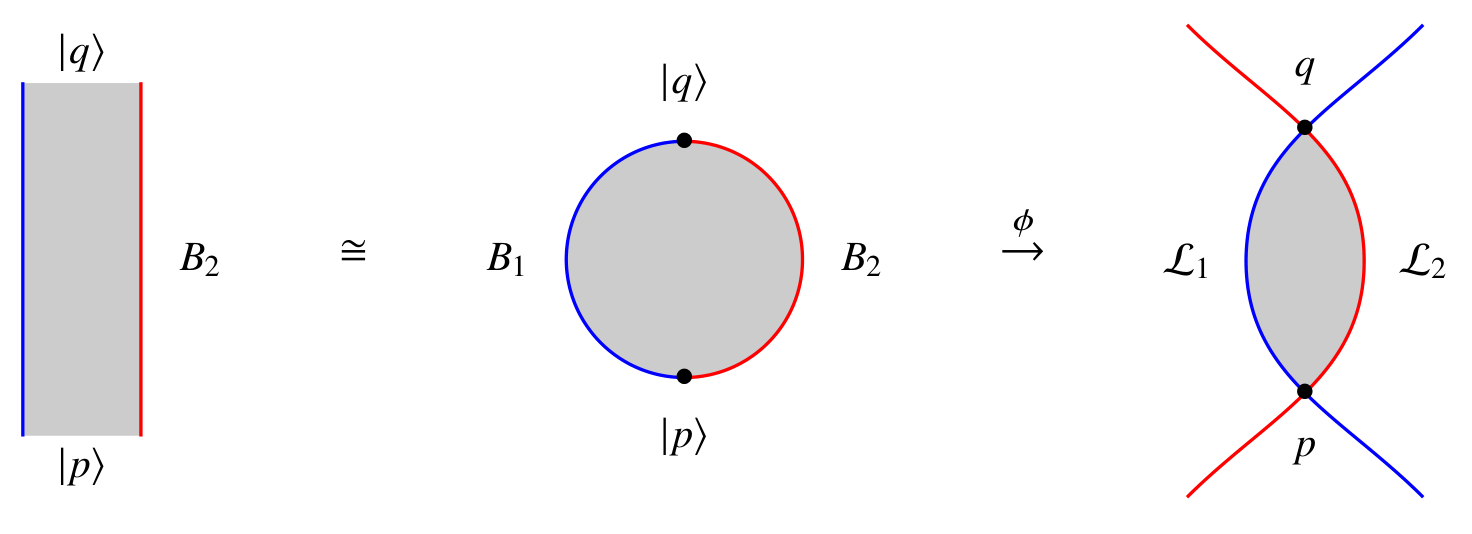
\includegraphics[width=0.92\linewidth]{figures/fig06.png}
  \caption{与从微扰基态 $|p\rangle$ 隧穿到微扰基态 $|q\rangle$ 相对应的瞬子修正的图示。在由手征多重态给出的映射 $\phi:\Sigma\to\mathcal{X}$ 下，该瞬子被解释为一个全纯圆盘，其边界落在拉格朗日（子流形）$\mathcal{L}_1,\mathcal{L}_2$ 上，而这两个拉格朗日（子流形）描述长条两个边界上的边界条件 $B_1,B_2$。（原文第 31 页，Figure 6）}
\end{figure}

这样的计数是否有意义并非显而易见——先验地，上述全纯圆盘的模空间可能有无限多个点！此外，$Q_A$ 是否为微分（即其平方是否为零）也不清楚。如附录 B 所述，$R$ 对称性所提供的 $\mathbb{Z}$ 分次恰好解决了这一困难。
% [跨页接续: 原文第30页/第31页——该句跨页（第 30 页末行 "the $\mathbb{Z}$-grading" 接第 31 页首行），已按语义完整置于此处]

% ==== 原文 PDF 第 31 页 ====
在有限维情形下，赋予超势的临界点 $p$（满足 $d_Mh(p)=0$）的 $\mathbb{Z}$ 分次由该点的 Morse 指标 $\mu(p)$ 给出。
% [原文疑误: 原文 "the Morse index $\mu(p)$ equal to the number of negative eigenvalues" 中缺少系动词 is（应为 "is equal to"）；译文按语义补足，符号与公式未改。]
显式地，Morse 指标 $\mu(p)$ 等于 Hessian 的负本征值个数。（假设 $h$ 的 Hessian 在每个临界点 $p$ 处非退化。总可以通过扰动 $h$ 使之如此。）如附录 B 所解释，Morse 指标对应于微扰基态 $|p\rangle$ 的 $R$ 荷。就梯度流而言，它计算的是「向下流动」方向的数目。由于超荷 $Q$ 的 $R$ 荷为 $+1$，只需考虑从临界点 $p$ 到满足 $\mu(q)=\mu(p)+1$ 的临界点 $q$ 的瞬子／Morse 流。

细致分析 Morse 流方程可以证明：在 $+\infty$（相应地 $-\infty$）处渐近于 $q$（相应地 $p$）的 Morse 流模空间，其（预期\footnote{我们指出，对常微分方程的分析把解模空间的预期维数给出为某个适当的 Dirac 算子的指标。然而，若 Morse 函数和／或度规退化，模空间的维数就可能偏离预期维数。经过适当的形变，可以使模空间的实际维数等于预期维数。}）维数为 $\mu(q)-\mu(p)$。于是当 $\mu(q)=\mu(p)+1$ 时，流模空间有无限多个点，但这在预料之中——总可以平移流的「时间」参数以得到另一个解。对这些平移取商之后可见，约化流模空间的（预期）维数为 0，即它只是若干个点。特别地，微分 $Q_A$ 只是带符号地计数这些点的数目：\footnote{关于这些微妙的符号问题，精确而细致的处理参见 [48, 附录 F]。}
% [Tutor Note: 这里「带符号计数」的来源是约化模空间的定向：0 维紧致定向流形是有限个带符号的点。符号约定依赖于定向的选取，文献中常用 $(-1)^{F}$ 的约定，跨文献比较时须先核对定向与符号规则。]
\begin{equation}\tag{2.50}
Q_A|p\rangle = \sum_{q,\ \mu(q)=\mu(p)+1}
\binom{\#\ \text{Morse 流}}{p\to q}|q\rangle
\end{equation}
% [Tutor Note: 该式即 Morse–Smale–Witten 复形的微分；二项式记号表示「从 $p$ 到 $q$ 的 Morse 流（连通分量）的带符号个数」，它只在 $\mu(q)-\mu(p)=1$ 时与微分有关。]

为检验这确实定义了微分，即 $Q_A^2=0$，需要（带符号地）计数从给定临界点 $p$ 到另一个满足 $\mu(r)=\mu(p)+2$ 的临界点 $r$、且经过第三个临界点 $q$（$\mu(q)=\mu(p)+1$）的流。注意从 $p$ 到 $r$ 的（约化）梯度流模空间具有（预期）维数 $2-1=1$。如附录所述，这一（约化）模空间的连通分支必然具有 $\mathbb{R}$ 的拓扑，而两端 $\pm\infty$ 恰好对应于这些复合流 $p\to q\to r$。特别地，给定的复合流

% ==== 原文 PDF 第 32 页 ====
$p\to q\to r$ 总与另一条符号相反的复合流 $p\to q'\to r$（其中 $\mu(q')=\mu(p)+1$）配对，因此这些复合流的总计数相消，即 $Q_A^2|p\rangle = 0$。
% [Tutor Note: 这里是 $Q_A^2=0$ 的标准配对论证：1 维模空间的两端给出符号相反的复合流，故成对相消；其严格性依赖 Morse–Smale 横截性与光滑紧化（附录 B 有详细讨论）。]

可以把这些论证形式地用于我们的 $A$ 型扭变 $\sigma$ 模型：微扰基态 $|p\rangle$ 由（横截相交的）拉格朗日（子流形）$\mathcal{L}_1,\mathcal{L}_2$ 的交点 $p\in\mathcal{L}_1\cap\mathcal{L}_2$ 标记；该交点的 Morse 指标由交点的 Maslov 指标给出；而 Morse 流方程对应于边界落在 $\mathcal{L}_1,\mathcal{L}_2$ 上的全纯长条／圆盘的映射。
% [原文疑误: 原文 "the Morse index of the the intersection point" 中 "the" 重复一次；译文只译一处，其余未改。]
% [Tutor Note: 这里的对应关系是 A 模型侧的字典：交点 $\leftrightarrow$ 微扰基态，Maslov 指标 $\leftrightarrow$ 分次，梯度流方程 $\leftrightarrow$ 带边全纯曲线方程（$\bar\partial u=0$ 加上拉格朗日边界条件）。]

由此得出结论：由（横截相交的）拉格朗日（子流形）$\mathcal{L}_1,\mathcal{L}_2$ 标记的边界条件之间的态射空间 $\operatorname{Hom}_{\mathbf{Bdy}_A}(B_1,B_2)$ 为
% [版式说明: 原文 (2.51) 为左右并置的两个式子共用同一个编号；此处因行宽所限排为上下两行，内容与编号均不变。]
\begin{equation}\tag{2.51}
\begin{gathered}
\operatorname{Hom}_{\mathbf{Bdy}_A}(B_1,B_2)
= H\Big(\bigoplus_{p\in\mathcal{L}_1\cap\mathcal{L}_2}|p\rangle,\ Q_A\Big)\\
Q_A|p\rangle = \sum_{q,\ \mu(q)=\mu(p)+1}
\binom{\#\ \text{全纯长条/圆盘}}{p\to q}|q\rangle\,.
\end{gathered}
\end{equation}

右端的复形称为 Floer 复形（Floer complex），其上同调称为 Floer 上同调。尽管 Floer 复形依赖于许多显式的选择，例如某个给定 哈密顿同痕类的具体代表元，但 Floer 上同调并不依赖这些选择。

给定三个拉格朗日（子流形）$\mathcal{L}_1$、$\mathcal{L}_2$、$\mathcal{L}_3$，它们两两横截相交，则 Floer 复形上存在一个自然的乘积结构，称为 Floer 乘积，它将给出 $A$ 型扭变下边界条件范畴中态射的复合。粗略地说，给定交点 $p_{12}\in\mathcal{L}_1\cap\mathcal{L}_2$、$p_{23}\in\mathcal{L}_2\cap\mathcal{L}_3$ 与 $q_{13}\in\mathcal{L}_1\cap\mathcal{L}_3$，$|p_{23}\rangle\star|p_{12}\rangle$ 中 $|q_{23}\rangle$ 的系数由带三个标记点的全纯圆盘的（带符号）计数给出：
% [原文疑误: 此处 "the coefficient of $|q_{23}\rangle$" 应为 $|q_{13}\rangle$——本段给出的交点为 $q_{13}\in\mathcal{L}_1\cap\mathcal{L}_3$，紧接的式 (2.52) 也是对 $q_{13}$ 求和并给出 $|q_{13}\rangle$ 的系数，第 33 页 Figure 7 的图注同样写 "the coefficient of $|q_{13}\rangle$"；译文照录原文的 $|q_{23}\rangle$。]
\begin{equation}\tag{2.52}
|p_{23}\rangle\star|p_{12}\rangle = \sum_{q_{13}}
\binom{\#\ \text{全纯圆盘}}{p_{12},p_{23}\to q_{13}}|q_{13}\rangle\,,
\end{equation}
其中求和遍历满足 $\mu(q_{13})=\mu(p_{12})+\mu(p_{23})$ 的交点 $q_{13}\in\mathcal{L}_1\cap\mathcal{L}_3$。图示见图 7 左。Floer 乘积在 Floer 上同调层面诱导出结合的复合，从而定义我们的 $A$ 膜范畴：对象是 Maslov 类为零（$\mu(\mathcal{L})=0$）的拉格朗日（子流形）$\mathcal{L}$（模去 哈密顿同痕），$\mathcal{L}_1$ 与 $\mathcal{L}_2$ 之间的态射由交集的 Floer 上同调给出，态射的复合由 Floer 乘积给出；所得范畴称为 $\mathcal{X}$ 的 Fukaya 范畴。
\begin{equation}\tag{2.53}
\mathbf{Bdy}_A \cong \operatorname{Fuk}(\mathcal{X})\,.
\end{equation}
% [Tutor Note: 到这一步，$A$ 侧与 $B$ 侧的范畴化已互为镜像：式 (2.47) 的 $D^b\operatorname{Coh}(\mathcal{X})$ 与式 (2.53) 的 $\operatorname{Fuk}(\mathcal{X})$ 分别是 $B$ 型与 $A$ 型扭变下边界条件范畴的数学表述，而同调镜像对称（HMS）断言它们（在镜像对 $(\mathcal{X},\check{\mathcal{X}})$ 上）是等价范畴。]

需要注意的是，Floer 乘积不满足结合律，但偏离方式受到高度控制。具体说，它在同伦意义下结合，或称同伦结合的（homotopy associative）。例如，给定四个拉格朗日（子流形）$\mathcal{L}_1,\ldots,\mathcal{L}_4$ 与 $Q_A$ 闭的交点 $p_{12},p_{23},p_{34}$，复合 $p_{12}\star(p_{23}\star p_{34})$ 与 $(p_{12}\star p_{23})\star p_{34}$ 之差，是某个（形式和的）交点 $\mu_3(p_{12},p_{23},p_{34})\in\mathcal{L}_1\cap\mathcal{L}_4$ 的 $Q_A$ 变分。示意地说，我们对连接这些固定点、且边界落在 $\mathcal{L}_1,\ldots,\mathcal{L}_4$ 上的全纯圆盘作（带符号的）计数：
% [Tutor Note: 这里要分清两件事：$\mu_3$ 的「取值」是 $\mathcal{L}_1\cap\mathcal{L}_4$ 上交点的一个形式线性组合（故式 (2.54) 右端对 $q_{14}$ 求和并带 $|q_{14}\rangle$），而结合律失效的程度正是这个组合；后者是 Massey 积在 Floer 理论中的实现。]
\begin{equation}\tag{2.54}
\mu_3(p_{12},p_{23},p_{34}) = \sum_{q_{14}}
\binom{\#\ \text{全纯圆盘}}{p_{12},p_{23},p_{34}\to q_{14}}|q_{14}\rangle
\end{equation}
其中求和遍历满足 $\mu(q_{14})=\mu(p_{12})+\mu(p_{23})+\mu(p_{34})-1$ 的交点 $q_{14}\in\mathcal{L}_1\cap\mathcal{L}_4$。图示见图 7 右。存在一整座高阶乘积 $\mu_n(p_{12},\ldots,p_{n\,n+1})$ 的塔，它由计数渐近趋于这些临界点的全纯圆盘得到；与 Floer 乘积 $\mu_2=\star$ 及三元乘积 $\mu_3$ 一起，这一族运算蕴含大量信息，并赋予 Fukaya 范畴 $A_\infty$ 范畴的结构。这些同伦的数据在下降（descent）的语言下有自然的物理解释，下一节将转向这一点。
% [跨页接续: 原文第32页/第33页——末句自第 32 页末行 "There is an entire tower of higher order products" 跨至第 33 页首行，已按语义完整置于本分片；故本分片含第 33 页页首的这一段。第 33 页页首的 Figure 7 归入 s03a.tex。]
% [Tutor Note: 塔 $(\mu_1=Q_A,\mu_2=\star,\mu_3,\ldots)$ 满足 $A_\infty$ 关系 $\sum_{i+j=n+1}(-1)^{\cdots}\mu_i(\ldots\mu_j(\ldots)\ldots)=0$；$\mu_1^2=0$ 给出微分，$n=3$ 的关系即「结合律只差同伦」，而更高阶 $\mu_n$ 全由全纯圆盘的计数确定。注意这里的 $\star$ 次序约定：$|p_{23}\rangle\star|p_{12}\rangle$ 对应先 $p_{12}$ 后 $p_{23}$ 的复合方向，核对 $A_\infty$ 关系中的符号时须与之一致。]
